\documentclass{article}

\usepackage[dvips]{graphicx}

\begin{document}

\title{Boolean Algebra in a Nutshell}

\author{Peter Mills}

\maketitle

\section{Introduction}

The usual approach to teaching logic is to start with Aristotelian logic.
In today's digital world, I think a more natural starting point for the
topic is Boolean algebra.
Not only does it flow more naturally into more modern logics such as propositional
and first-order logic, it is also invaluable to both the computer programmer
and computer engineer.

Let $P$ be a proposition, for instance, ``{\it Roses are red},''
``{\it The sky is blue},'' or ``{\it All dogs are mammals}.''
As such, $P$ will take on a truth value.
In Boolean logic, it may take on only one of two values: 
that is, it is either true or false, $0$ or $1$; $P \in \lbrace 0, ~ 1 \rbrace$.

The purpose of Boolean algebra is to form conjunctive expressions with one or
more of these propositions.
On the basis of the truth values of the individual propositions, the truth
of the entire expression may be evaluated.

Two of the most common conjunctions used in English to unite two or more
statements (propositions) are AND and OR, for instance:
\begin{quote}
	{\it Roses are red} AND {\it the sky is blue}.
\end{quote}
These conjunctions are also used in Boolean logic as {\it operators} between
two propositions,
although OR is somewhat different than how it is used in English.

The two symbols for AND and OR are $\land$ and $\lor$, respectively.
Suppose we have two propositions, $P$ and $Q$.
We can use these operators to unite them, thereby turning them into a new
proposition:
\begin{equation}
	P \land Q
\end{equation}
which is read, ``$P$ AND $Q$''.
Another useful operator is the NOT or negation operator, $\lnot$.
This is a {\it unary} rather than a {\it binary} operator, hence operates on
only one argument:
\begin{equation}
	\lnot P
\end{equation}

An interesting feature of Boolean logic, is that unlike in older forms of logic,
such as Aristotelian logic, the entire content of an elementary proposition,
such as $P$, above, is abstracted away, leaving only the binary truth value.


\begin{table}
	\caption{List of operators used in Boolean algebra.
All operators return a new binary proposition.}
\begin{tabular}{lll}
	Name & Symbol & Example \\
	\hline
	AND & $\land$ & $X \land Y$ \\
	OR & $\lor$ & $X \lor Y$\\
	NOT & $\lnot$ & $\lnot X$ \\
	if-then & $\rightarrow$ & $X \rightarrow Y$ \\
	if-and-only-if & $\iff$ & $X \iff Y$ \\
	exclusive OR (XOR) & $\oplus$ & $X \oplus Y$ \\ 
	\hline
\end{tabular}
\end{table}

\section{Truth tables}

As mentioned in the previous section, combining one or more propositions with
an operator creates a new proposition.
How do we determine the truth value of this new proposition?
One way is using a {\it truth table}.
A truth table tabulates the truth value of the whole expression for every possible
truth value of each of the consituent propositions.

Here is the {\it truth table} for the AND operator:

\begin{tabular}{ll|c}
	$X$ & $Y$ & $X \land Y$ \\
	\hline
	0 & 0 & 0 \\
	0 & 1 & 0 \\
	1 & 0 & 0 \\
	1 & 1 & 1 \\
\end{tabular}

Note that the logical OR is different from the English ``or''.
In English speech, ``or'' is the equivalent to the exclusive OR (
XOR) which will be discussed in next section.

\begin{tabular}{ll|c}
	$X$ & $Y$ & $X \lor Y$ \\
	\hline
	0 & 0 & 0 \\
	0 & 1 & 1 \\
	1 & 0 & 1 \\
	1 & 1 & 1 \\
\end{tabular}

NOT is logical negation:

\begin{tabular}{l|c}
	$X$ & $\lnot X$ \\
	\hline
	 1 & 0 \\
	 0 & 1 \\
\end{tabular}

\section{Gates and logic circuits}

\begin{table}
	\caption{Table of gates and equivalent Boolean expressions.}\label{gates}
	\begin{tabular}{|c|c|c|}
		\hline
		Name & gate & expression \\
		\hline\hline
		AND & 
\includegraphics{and_gate.eps} & $X \land Y$\\
		\hline
		OR & 
\includegraphics{or_gate.eps} & $X \lor Y$\\
		\hline
		NOT & 
\includegraphics{not_gate.eps} & $\lnot X$\\
		\hline
		NAND & 
\includegraphics{nand_gate.eps} & $\lnot(X \land Y)$\\
		\hline
		NOR & 
\includegraphics{nor_gate.eps} & $\lnot(X \lor Y)$\\
		\hline
		XOR & 
\includegraphics{xor_gate.eps} & $X \oplus Y$\\
		\hline
	\end{tabular}
\end{table}

\begin{figure}
	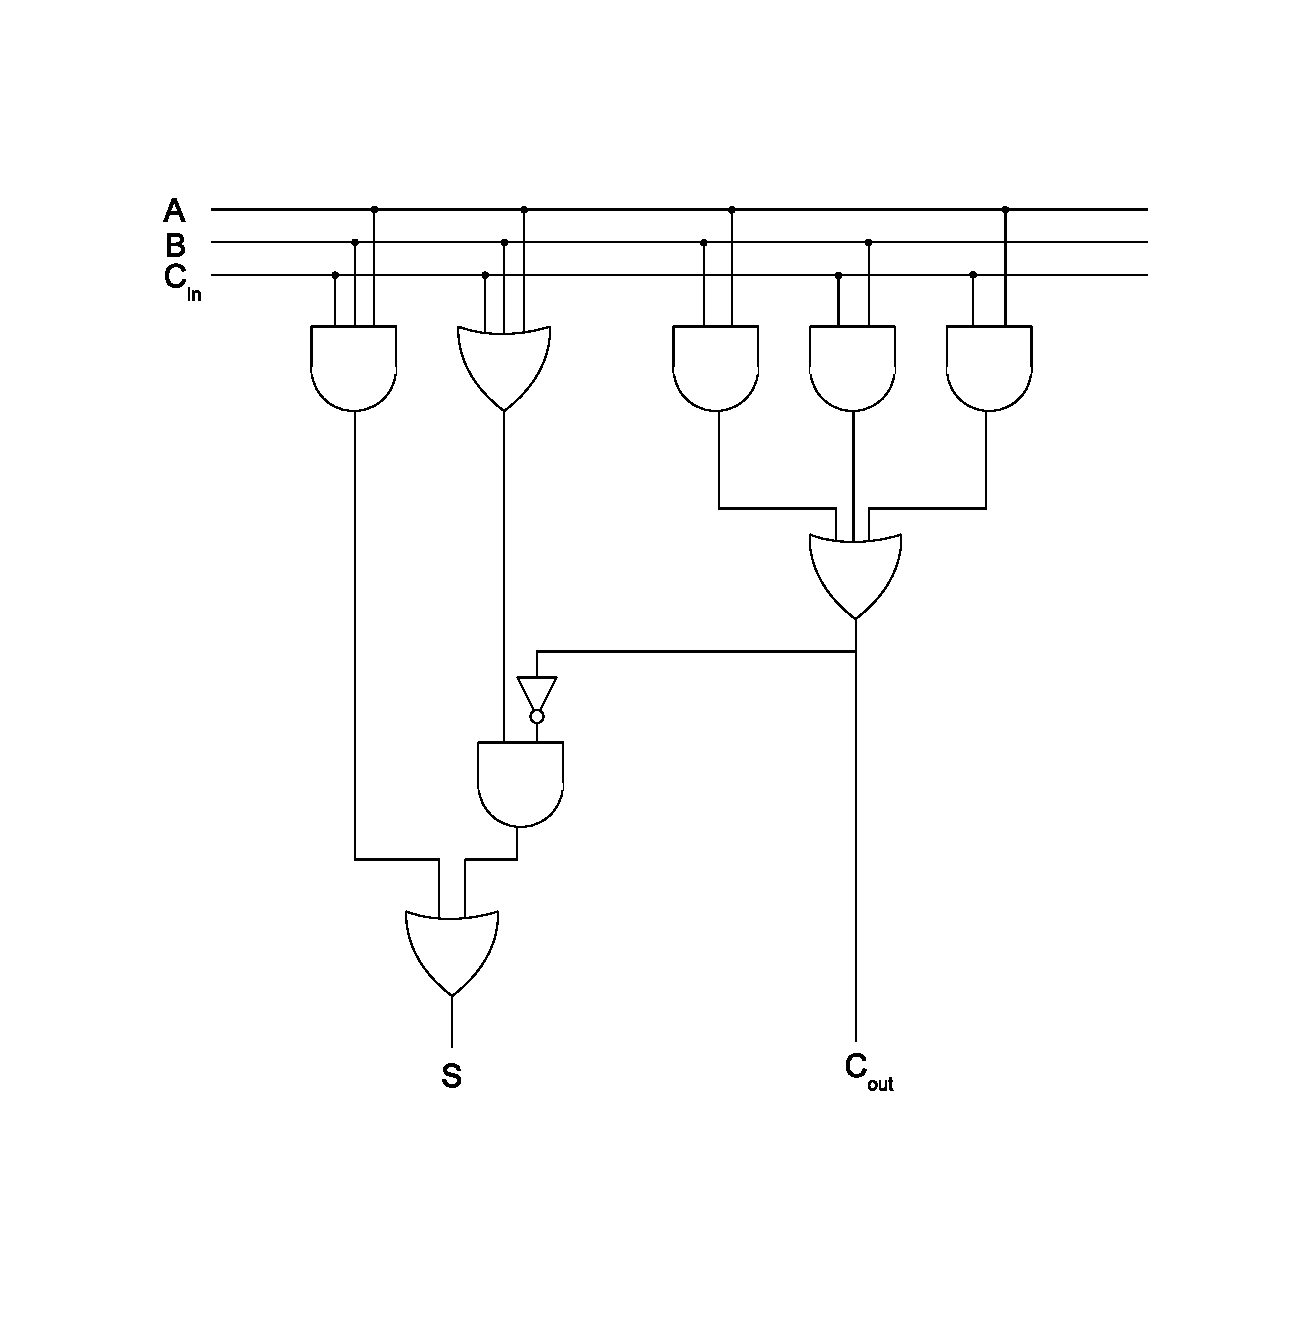
\includegraphics[width=1\textwidth]{adder.eps}
	\caption{Logic circuit for a binary adder.}\label{adder}
\end{figure}

Any Boolean expression can be written as a logical circuit network using
{\it gates}.
Table \ref{gates} lists the gates and their equivalent Boolean operations. 

Consider the following pair of expressions:
\begin{eqnarray}
	(A \land B \land C_{in}) \lor \left \lbrace (A \lor B \lor C_{in}) \land \lnot \left [(A \land B) \lor (B \land C_{in}) \lor (A \land C_{in}) \right ] \right \rbrace \\
	(A \land B) \lor (B \land C_{in}) \lor (A \land C_{in})
\end{eqnarray}
This is a {\it binary adder} and the equivalent logic circuit is shown
in Figure \ref{adder}.
The first expression is the sum ($S$) and the second is the {\it carry bit} ($C_{out}$).
Note how the circuit allows repeated expressions to be re-used without
needing multiple versions.

A set of adders lined up in series with each ``carry out'' bit ($C_{out}$)
routed to the next ``carry in'' bit ($C_{in}$) can be used to add multiple
digit binary numbers.


\section{Tautologies and logical implication}

A {\it tautology} is an expression that is always true.
Consider for instance:
\begin{equation}
	P \lor \lnot P
\end{equation}

Now, consider these two new operators: logical implication 
or if-then ($\rightarrow$) and if-and-only-if ($\iff$).

If $X$ then $Y$ ($X \rightarrow Y$) is defined:

\begin{tabular}{ll|c}
	$X$ & $Y$ & $X \rightarrow Y$ \\
	\hline
	0 & 0 & 1 \\
	0 & 1 & 1 \\
	1 & 0 & 0 \\
	1 & 1 & 1 \\
\end{tabular}

This is equivalent to $\lnot X \lor Y$.

To define if-and-only-if, we first define the exclusive OR or XOR 
which is as follows:

\begin{tabular}{ll|c}
	$X$ & $Y$ & $X \oplus Y$ \\
	\hline
	0 & 0 & 0 \\
	0 & 1 & 1 \\
	1 & 0 & 1 \\
	1 & 1 & 0 \\
\end{tabular}

If-and-only-if, $\iff$, is simply a negated XOR ($\lnot (X \oplus Y)$).

Now consider two equivalent expressions, for instance $X \rightarrow Y$
and $\lnot X \lor Y$, above.
We can write:
\begin{equation}
	(X \rightarrow Y) \iff (\lnot X \lor Y)
\end{equation}
This expression is a tautology
It also encapsulates a {\it rule-of-inference},
that is you can substitute the expression on the left for the one on the right
and vice versa.

For the one way case, where you can substitute the expresson on the left
for the one on the right, but not the other way around, we use if-then.
For example:
\begin{equation}
	(X \iff Y) \rightarrow (X \rightarrow Y)
\end{equation}


\section{Boolean logic and computational complexity}

Boolean algebra is important in computational complexity theory.
Satisfying a Boolean expression is a prototypical NP-complete problem.
The worst-case running time to find a set of inputs that returns a value of 1
increases exponentially with the number of inputs.
This is the meaning of NP or ``non-polynomial''.
Moreover, other NP problems are equivalent to this problem and all such 
equivalent problems are ``NP-complete''.

The most discussed NP-complete problem is the travelling salesmen problem,
which is as follows: given a set of points, what is the shortest path that
passes through all of them?
Note that in this context, it must be formulated as a decision problem:
that is, given a set of points and a distance threshold, find a path that
is less than the threshold.
Presumably, one could design a network that would accurately model any given
travelling salesment problem.

While any potential solution can be verified in polynomial time--the
running time is proportional to the size of the network--finding a solution
can currently only be acheived in non-polynomial time--the running time
is proportional the exponent of the size.
It is currently an unsolved problem whether algorithms exist that can
find a solution to NP-complete problems in polynomial time.

\section{Exercises}

\begin{enumerate}
\item
\begin{enumerate}
	\item Derive the truth table for NOR and NAND.
	\item Write all the gates and operators in terms of NOT and NOR.
	\item Write all the gates and operators in terms of NOT and NAND.
\end{enumerate}
	\item
\begin{enumerate}
	\item Derive the truth table for the binary adder. Hint: here I've started it off for you,

		\begin{tabular}{lll|ll}
			$A$ & $B$ & $C_{in}$ & $S$ & $C_{out}$ \\ \hline
			0 & 0 & 0 & 0 & 0\\
			0 & 0 & 1 & & \\
			0 & 1 & 0 & & \\
			0 & 1 & 1 & & \\
			1 & 0 & 0 & & \\
			1 & 0 & 1 & & \\
			1 & 1 & 0 & & \\
			1 & 1 & 1 & &
		\end{tabular}

	\item See if you can come up with your own formulation for the adder.
		In particular, try to minimize the number of gates.
		The example uses a total of nine (9) gates. 
		Can you invent one that uses fewer?
\end{enumerate}
	\item
Prove the following tautologies (hint: once you have proven one tautology, you can use
it to help prove the others):
\begin{enumerate}
	\item $\lnot(A \land B) \iff (\lnot A \lor \lnot B)$
	\item $\lnot (A \lor B) \iff (\lnot A \land \lnot B)$
	\item $\left [ A \land (B \lor C) \right ] \iff \left [ (A \land B) \lor (A \land C) \right ]$
	\item $\left [A \lor (B \land C)\right ] \iff \left [ (A \lor B) \land (A \lor C) \right ]$
\item $\left [ (A \rightarrow B) \land (B \rightarrow A) \right ] \iff (A \iff B)$
\end{enumerate}
\end{enumerate}


\end{document}

